%!TEX root = ../main.tex
%%%%%%%%%%%%%%%%%%%%%%%%%%%%%%%%%%
% Links:
%
% Difficulty: Easy/Medium Companies: 
%%%%%%%%%%%%%%%%%%%%%%%%%%%%%%%%%%

%\chapterimage{header}

\chapter{Power set generation}
\label{ch:power_set}
\section*{Introduction}

Most readers will already be familiar with power sets, i.e.  the set of all the subsets of a set $S$.  Being asked to generate the power set of a given set, both directly and indirectly, is a frequently asked question in coding interviews and therefore, in this chapter, we will investigate  two different solutions.  

\begin{enumerate}
    \item The first approach derives straightforwardly from the recursive definition of power-set, which states "the power-set of an empty set is a set containing one element only: the empty set itself". 
    For a non-empty set $S$, let $e$ be an element of $S$ and $T$ be the original set $S$ set minus $e$ ( $T=S \setminus e$), then the power set of $S$ is defined as the union of two distinct power sets:
    \begin{itemize}
        \item   the power set of $T$
        \item   and the power set of $T$ modified in a such way that $e$ is added to all of its elements (See Equation \ref{eq:power_set_recursive_definition}).  
    \end{itemize}
    \item The second approach is based on a bit-distribution property in the integers binary representation from $0$ to the size of the power set.

\end{enumerate}

The two proposed solutions have similar performance in terms of time space required, but the latter is easier to explain and results in shorter and simpler code. 

\begin{equation}
    \mathcal{P}(S)=\begin{cases} 
    \{\{\}\} & \text{if } S=\{\} \\
    \mathcal{P}\{T\} \bigcup \{t \bigcup \{e\} \: : t \in \mathcal{P}\{T\}\} \text{ where }  T = S \setminus \{e\} \text{ } \forall e \in S, & \text{otherwise}
    \end{cases}
    \label{eq:power_set_recursive_definition}
\end{equation}



\section{Problem statement}
    \begin{exercise}
        Write a function that given a set $S$ returns its power set.
The power-set of $S$ ($\mathcal{P}(S)$) is the set of all its subsets including the empty subset ($\emptyset$) and $S$ itself.

        \begin{example}
            \label{ex:power_set:example1}
            \hfill \\
            Given the set $S=\{a,b,c\}$, the following is a correct output for
            this problem: $$\{\{\}, \{a\}, \{b\}, \{c\}, \{a,b\}, \{b,c\}, \{a,c\}, \{a,b,c\} \}$$
        \end{example}
    \end{exercise}

\section{Clarification Questions}

\begin{QandA}
    
    \item  \begin{questionitem} \begin{question} What is the maximum input size?  \end{question}      
    \begin{answered}
           \textit{The maximum number of elements in $S$ is strictly less than $32$.}
        \end{answered} \end{questionitem}
    
    \item \begin{questionitem} \begin{question} Are all the elements in the collection distinct?  \end{question}
    \begin{answered}
        \textit{No, the elements are not necessarily distinct. $S$ might contain duplicates.}
    \end{answered} \end{questionitem}

    \item \begin{questionitem} \begin{question} Can the elements of the power-set appear in any order?  \end{question}
    \begin{answered}
        \textit{Yes, subsets can appear in any order. 
        For example the following is also a valid output for the input shown in Example \ref{ex:power_set:example1}:} 
        $\{\{\}, \{b,c\}, \{a\}, \{a,b\}, \{a,b,c\}, \{b\}, \{a,c\}, \{c\} \}$
    \end{answered} \end{questionitem}
\end{QandA}

\section{Discussion}
\label{sec:powerset:discussion}

The first key point to note is that the power set of a collection of $n$ elements has size $2^n$. The proof is straightforward and based on the fact that a subset of $S$ can be uniquely identified by a list $X=\{x_0,x_1,\ldots x_{|S|-1}\}$ of $|S|$ binary variables each carrying the information about whether $S_i$ is part of the subset; the variable $x_i$ is crucial to answer the question \textbf{should $S_i$ be part of this subset?}: If $x_i$ is true the answer is yes, otherwise, the answer is no.
We have two possible choices for every element of $S$ (either take it or not), then the total number of distinct $X$s  is: $2 \times 2 \times \ldots \times 2 = 2^{|S|}$. Two choices for the first element, two for the second, and so 
on until the last element of $S$.
  
This, together with the constraint on $|S|$ ($|S| < 32)$ is a strong indicator that an \textbf{exponential time and space} solution is expected.
After all, we are required to output all the elements of the power set, and thus the number of operations of an algorithm designed for this task cannot be less than the size of the power set itself. 



\subsection{Bruteforce - Backtracking-like approach}

The first approach to solving this problem is based on the fact that,  during the generation of
one of the power set's elements, a decision must be made for each element $e$ of $S$, on whether or not to include $e$ into the subset.
Once this is determined, what we are left with are $|S|-1$ decisions
before we have created a valid subset of $|S|$.

This process is inherently recursive and therefore easily visualized with a tree (see the figure below): a node at level $i$
represents a decision for the $i^{th}$ element of $S$ and a path from the root to a leaf uniquely
identifies a subset of $S$; after having traversed all the levels down to a leaf, $n$ decisions have been made: 
one for each of the elements of $S$. 

Collectively, all the paths from the root to the leaves are the power set, and therefore, in
order to solve the problem, we have to visit the entire tree.


A common route to solving such problems is to use a backtracking-like approach in order to try all possible
decisions (or equivalently to visit every path from the root to a leaf).

The idea is that, for all elements of $S$, from the first to the last one, we are going to
explore the two available possibilities: either take or exclude
it from the subset.

We start by making a decision for the first element: From there, we continue to generate all possible subsets
where the first decision is never changed. 
When there are no more subsets to generate, we *backtrack* and change our first
decision and repeat the process of generating all possible subsets.


For instance, given $S=\{1,2,3\}$, we might start by deciding to use the element $1$, and include it in all possible subsets from the remaining elements $\{2, 3\}$ only. 
Once we are done with it, we can repeat the same process, only this time excluding $1$. What we do is: $\mathcal{P}(S)= \{\{1\} \; \bigcup \;\mathcal{P}(\{2,3\})\} \: \bigcup \: \{\mathcal{P}(\{2,3\})\}\} 
$

The proposed solution will incrementally construct one subset at a time, 
using an integer variable to keep track of which element we are currently taking the decision for.
This type of problem is naturally solved recursively, with a base case of the recursion happening when there is no more decision
to make, meaning that the current subset is ready to be included in the solution (it has been
produced after $n$ decision steps).

Here below we can see how the \CC code implements this idea. The complexity of this solution is exponential i.e. $O(2^{|S|})$ which as already stated, is as good as
it gets.


\lstinputlisting[language=c++, caption="\CC to the power set generation using backtracking",label=list:power_set_backtracking]{sources/power_set/power_set_backtracking.cpp}


\begin{figure}
    \centering
    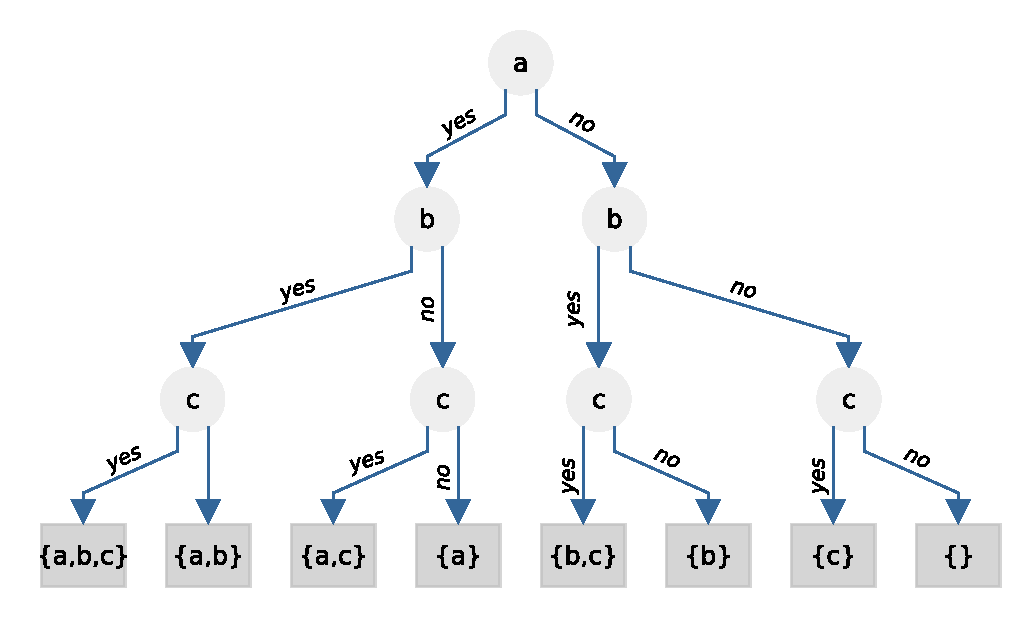
\includegraphics[width=\textwidth]{sources/power_set/images/tree}
    \caption[Decision tree for the power-set generation using backtracking.]{Decision tree for the power-set generation using a backtracking-like brute-force approach. At level $i$ are the decisions for the element $i$ in $S$. A label marked with "yes" identifies the decision to add the corresponding element into the subset, while a node labeled with "no" identifies the opposite. Each path from the root to a leaf is an element of the power set. At the last level is the power set.}
    \label{ref:power_set_decision_trees}
\end{figure}

Using a backtracking-like approach is convenient because, once we identify that a problem can be solved by fully exploring the associated search space tree, we can immediately
start writing the code and rely on our experience as backtracking expert writers to implement a correct
solution. It is also concise and short when written in a recursive  form (fewer chances to make mistakes, and less code to debug and explain),  as well
as easily understood.
The downside is that, if we decide to use it, an iterative implementation can be a little harder and verbose to write.

Regardless of which type we decide to write, the interviewer will be pleased with the code provided,  although it remains important to get to the final solution
without making too many implementation mistakes such as forgetting to handle the base case.


\subsection{Bit Manipulation}

The second approach to solving this problem is based on the fact that the values of the
bits of the numbers $\{0,1,2,\ldots, s^n-1\}$  already provide all the information necessary to decide whether or not to include an element from $S$ into a subset. 
The main principle is that the binary representation of all the numbers ($2^{|S|}$ of them) from $0$ to $2^{|S|}-1$ is the power set of $n$ bits.
This means that the binary representation of any of those numbers carries the necessary information that can be used to build one subset of $\mathcal{P}(S)$. 


For example, given the input $S=\{a,b,c\}$ the table below shows numbers from $0$ to $2^3-1 = 7$ and their binary
representation (second column), as well as how the information about which bit is set can be used to construct one subset of $\mathcal{P}(S)$ (third column).
\textbf{When the $i^{th}$ bit is set (its value is $1$), it means that
corresponding $i^{th}$ element of $S$ is chosen, while an unset bit (with value $0$) means it is
excluded}

\begin{table}
    \centering
    \begin{tabular}{|l|l|l|}
        \hline
        Number Value & Bits & Subset\\ \hline
        0     & 000  & $\{\}$\\ \hline
        1     & 001  & $\{c\}$\\ \hline
        2     & 010  & $\{b\}$\\ \hline
        3     & 011  & $\{b,c\}$\\ \hline
        4     & 100  & $\{a\}$\\ \hline
        5     & 101  & $\{a,c\}$\\ \hline
        6     & 110  & $\{a,b\}$\\ \hline
        7     & 111  & $\{a,b,c\}$ \\ \hline
    \end{tabular}
    \caption[Mapping between bits and element of the power set.]{This table shows a 1-to-1 mapping between integer values, their binary representation and an element of the power set.}
    \label{tab:mapping_value_bits}
\end{table}


This can be used to write an algorithm in which all the numbers in the range $\{0,1,2,\ldots,
2^{|S|}-1\}$ are considered and each of them is used to generate a subset of the final solution.
Every number from this range maps uniquely to a subset of $\mathcal{P}(S)$. 

The approach is easily understood when we think about the meaning of a bit in the binary representation of integers. One
can "build" a number $k$ by summing up powers of $2$ where the bits contain the information about whether a
certain power of two should be added to the final value. With $n$
bits one can represent $2^n$ numbers, each corresponding to one and only one subset of the power set of those $n$ bits.
Listing \ref{list:power_set_bits} shows  a possible \CC implementation of the idea above.

\lstinputlisting[language=c++, caption="Solution using bit manipulation.",label=list:power_set_bits]{sources/power_set/power_set_bit_manipulation.cpp}


The complexity of this function is, not surprisingly, $O(2^{|S|})$. 
We also pay a constant price of $32$ for each number we loop through given that we need to inspect all of its bits.
This proposed implementation assumes that the size of \inline{int} is $4$ bytes, which is true for most systems.

It is important to note the usage \inline{std::reserve} as it should be used in all those scenarios when we already know the final size of the collection we are building.
This saves time because it avoids intermediate allocations and copies that must happen during the resize of the vector.







%\section{Common variations}

%\section{Conclusion}
